\documentclass[a4paper, titlepage]{scrartcl}

\usepackage[ngerman]{babel}
\usepackage[utf8]{inputenc}
\usepackage[T1]{fontenc}
\usepackage{graphicx}

\title{UML Dokumentation}
\author{Damien Flury}
\date{27. Februar 2019}

\begin{document}
    \maketitle
    \tableofcontents
    \newpage
    \section{Einführung}
    \section{Vererbung}
    Bei der Vererbung (engl. Inheritance) von Klassen werden Unterklassen generalisiert. Java
    verfügt im Gegensatz zu zum Beispiel C++ nur über Single Inheritance, das heisst, dass eine Klasse
    jeweils nur von maximal einer anderen Basisklasse erben kann. Dies führt zu einigen Limitierungen,
    vereinfacht den Code jedoch. Somit muss in Java gegebenenfalls auf andere Beziehungen gesetzt werden,
    wie zum Beispiel die Komposition. Für grafische Beispiele siehe Abbildung \ref{VererbungDrawIO}
    und Abbildung \ref{VererbungUmlDesigner}
    \begin{figure}
        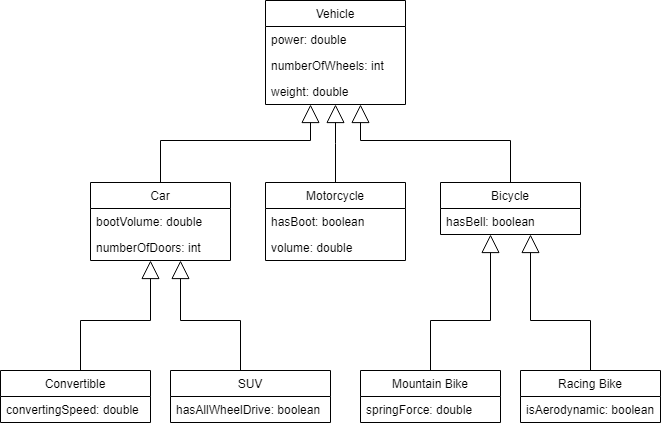
\includegraphics[width=\textwidth]{Klassendiagramm1a}
        \caption{UML-Diagramm mit Vererbung (draw.io)}
        \label{VererbungDrawIO}
    \end{figure}
    \begin{figure}
        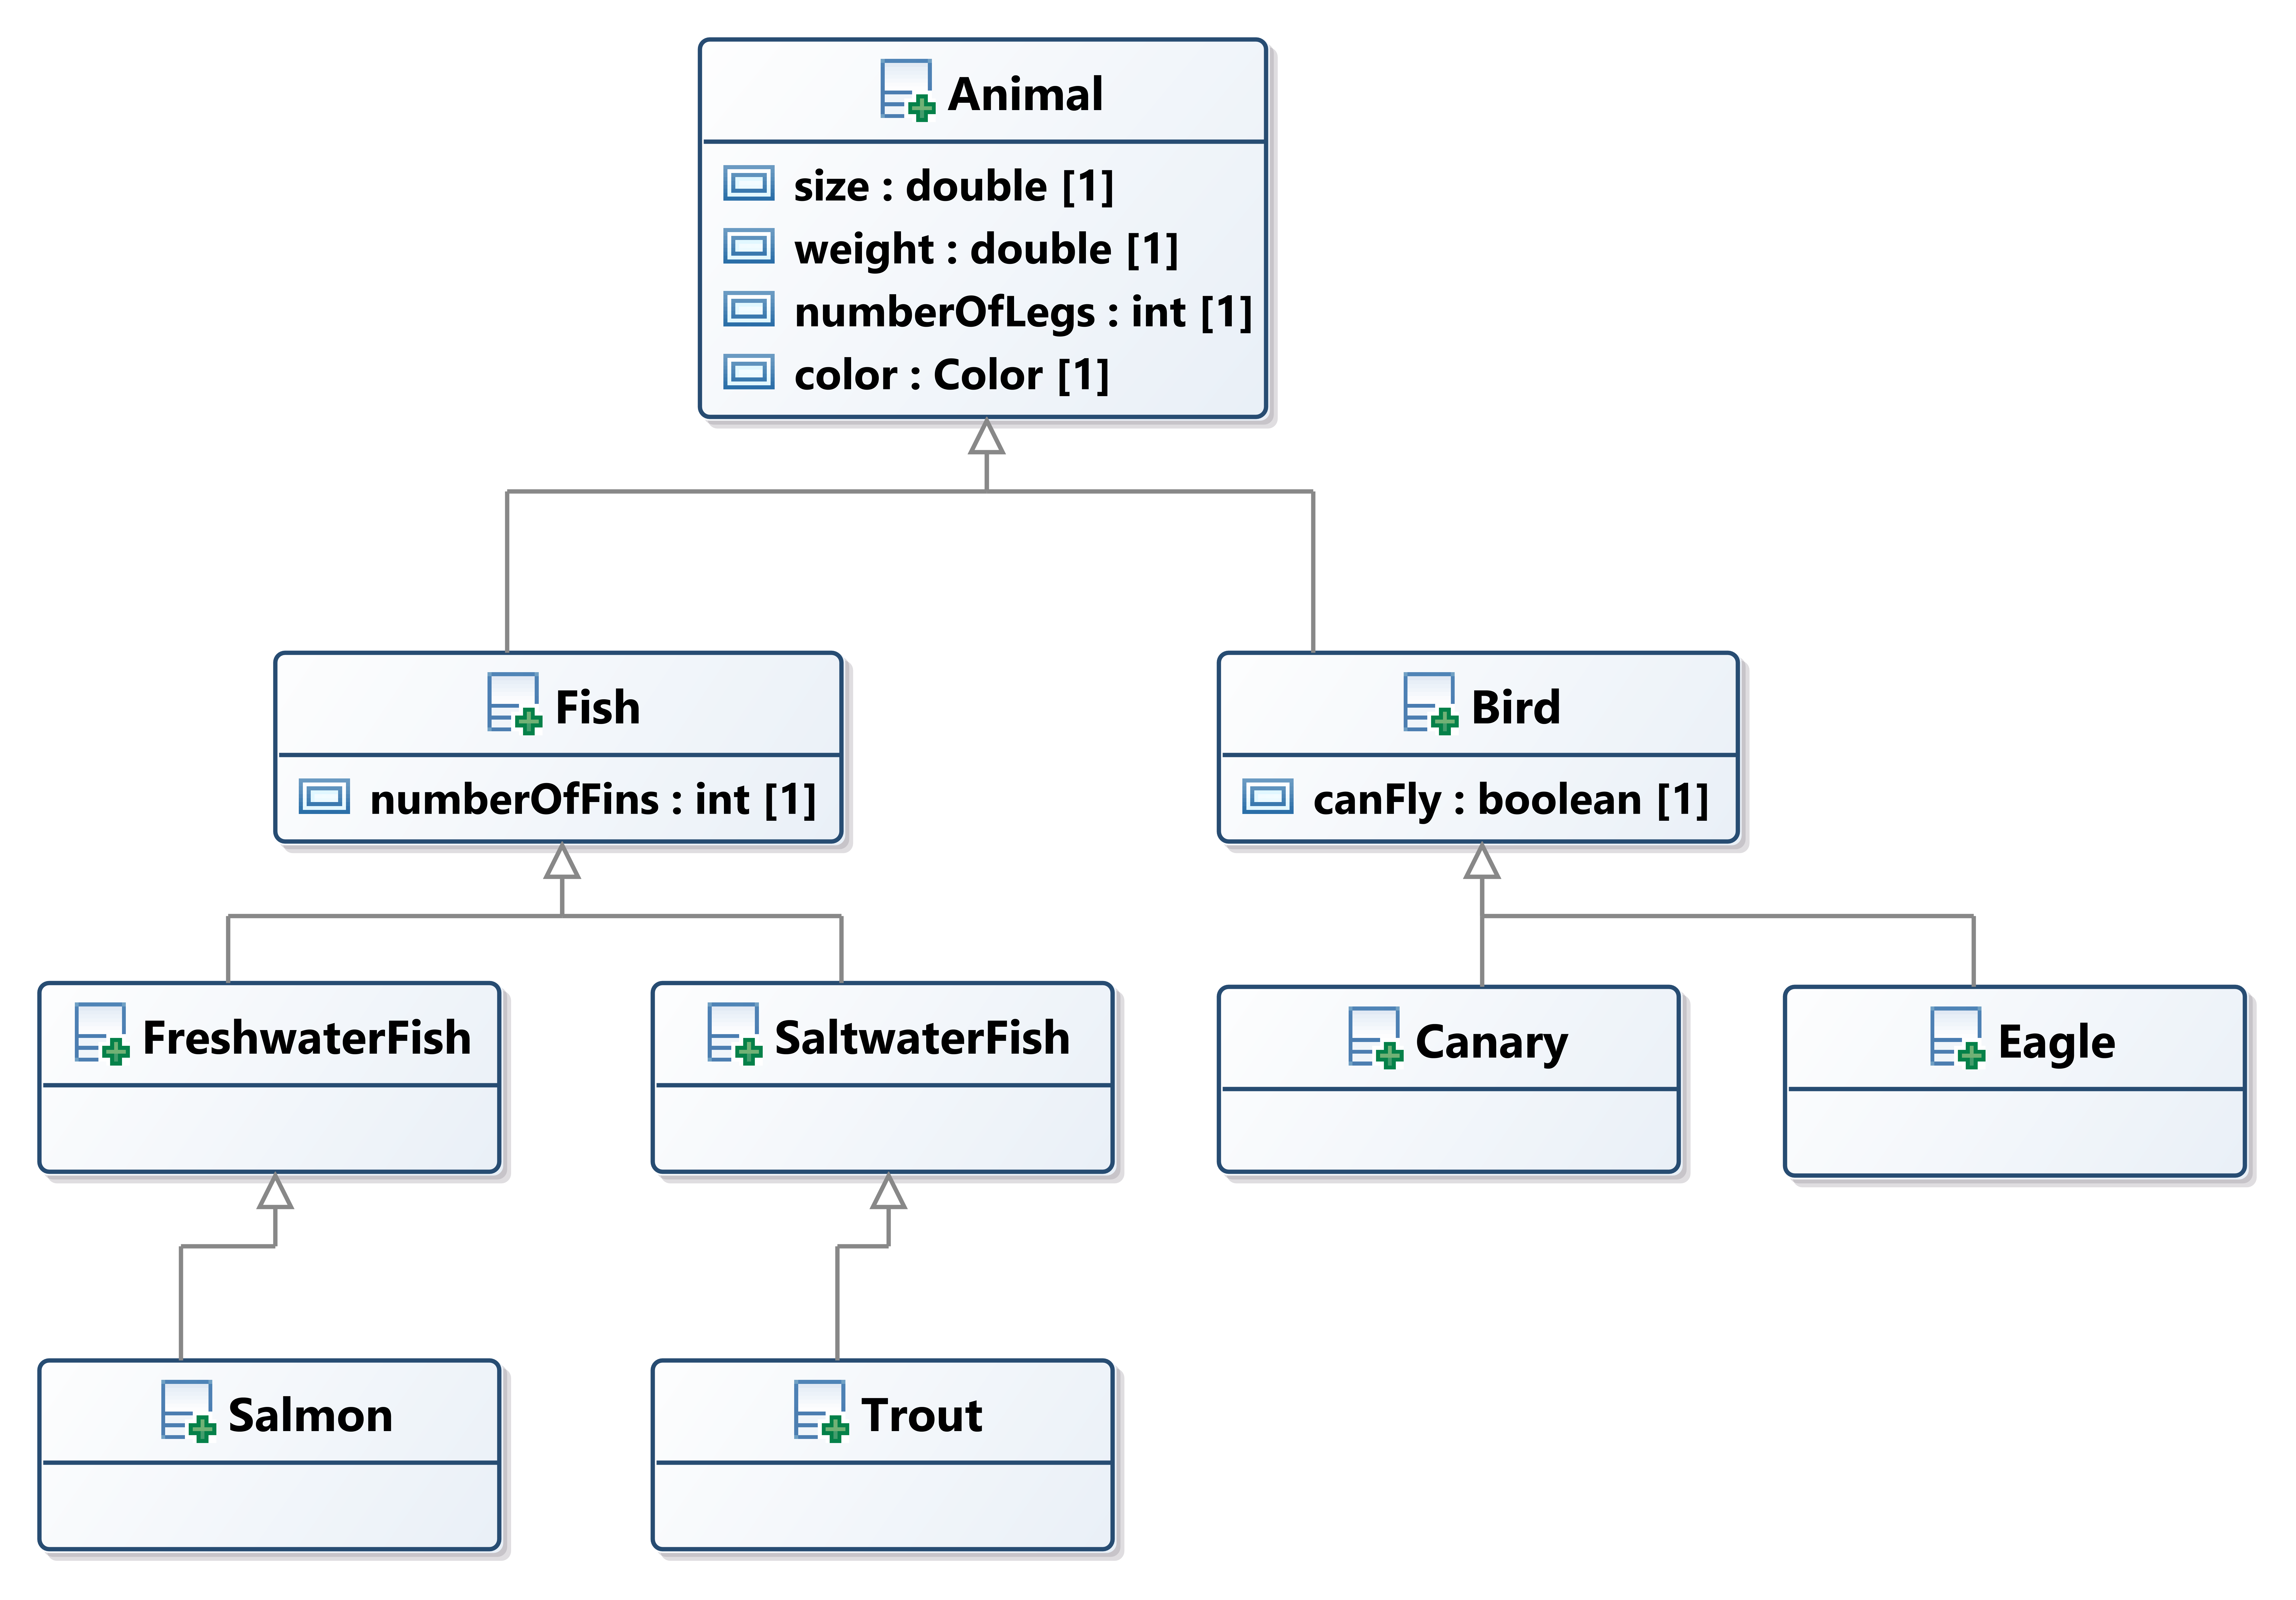
\includegraphics[width=\textwidth]{Klassendiagramm1b}
        \caption{UML-Diagramm mit Vererbung (UML Designer)}
        \label{VererbungUmlDesigner}
    \end{figure}
    
    \section{Assoziationen}
    Beim Assoziationsdiagramm geht es um Haben-/Kennenbeziehungen Siehe Abbildung \ref{AssoziationenDrawIO}
    \begin{figure}
        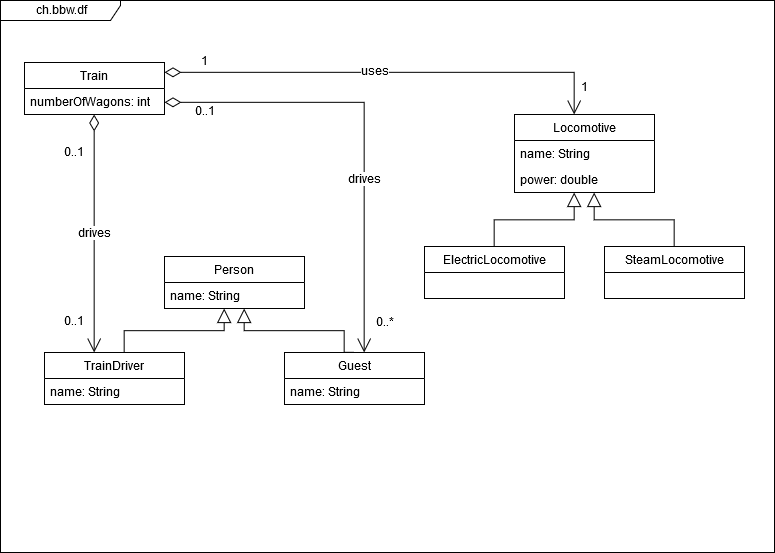
\includegraphics[width=\textwidth]{Assoziationen.png}
        \caption{Klassendiagramm mit Assoziationen (draw.io)}
        \label{AssoziationenDrawIO}
    \end{figure}

    \section{Use Case Diagram}
    Im Use Case Diagram werden verschiedene Funktionen aufgezeichent. 
    Beispiele: Abbildung \ref{UseCaseDrawIO} und Abbildung \ref{UseCaseVisio}
    \begin{figure}
        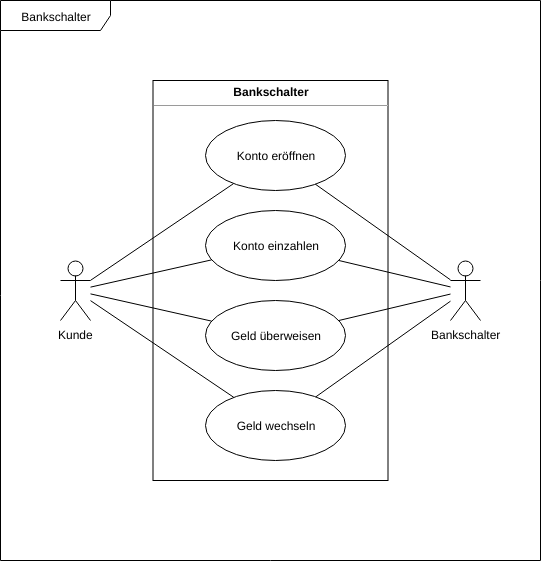
\includegraphics[width=\textwidth]{Anwendungsfalldiagramm1a.png}
        \caption{Use Case Diagram (draw.io)}
        \label{UseCaseDrawIO}
    \end{figure}
    \begin{figure}
        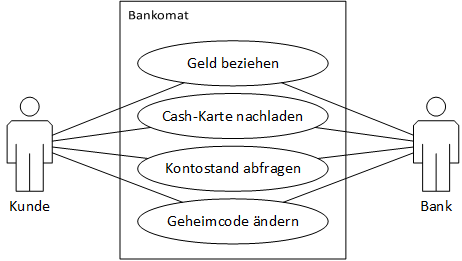
\includegraphics[width=\textwidth]{Anwendungsfalldiagramm1c.png}
        \caption{Use Case Diagram (Microsoft Visio)}
        \label{UseCaseVisio}
    \end{figure}

    \section{Aktivitätsdiagramm}
    Das Aktivitätsdiagramm zeigt eine Aktivität an. 
    Beispiel: Abbildung \ref{AktivitaetsdiagrammDrawIO}
    \begin{figure}
        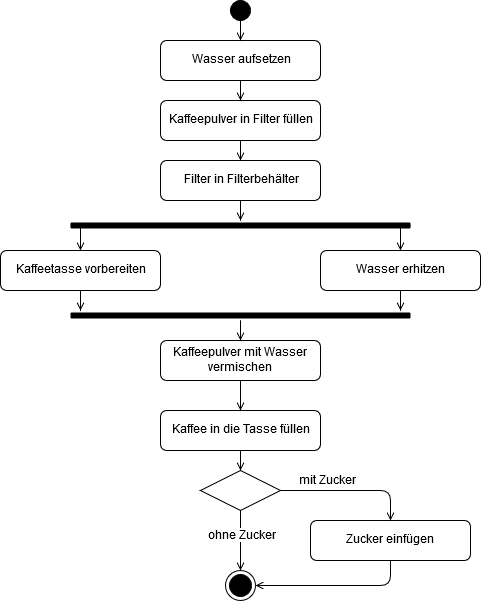
\includegraphics[width=\textwidth]{Aktivitaetsdiagramm1a.png}
        \caption{Aktivitätsdiagramm (draw.io)}
        \label{AktivitaetsdiagrammDrawIO}
    \end{figure}
    
\end{document}